\subsection{\label{sec:A1}Dark field microscopy}
Before delving into the qualitative analysis of the captured sample images, 
we provide a detailed description of the adjustment process. 
Initially, the sample must be shifted into the focus of the first objective. 
This adjustment is achieved by finely manipulating the sample stage using small knobs, 
allowing precise movement in all three spatial directions. 
The light reflected from the sample is directed onto the adjustable camera via a beam splitter, 
positioned above the light source for this initial step. 
The sample stage is finely adjusted until the nanorod sample fields are distinctly visible 
in sharp focus on the transmitted image. \\
Subsequently, the camera can be relocated to the position shown 
in Fig.~\ref{fig:aufbau}. 
In this configuration, the camera captures the light transmitted through the sample. 
The rear objective is adjusted to render the displayed image sharp. 
As a result, the sample is now in focus for both objectives. \\
At this point, a dark-field mask can be introduced into the optical path, 
preventing excitation light from reaching the second objective. 
Nevertheless, a signal corresponding to the scattered light from the nanoparticles is still 
detected on the camera. 
By inserting a polarizer, the unpolarized light can be linearly polarized, 
with the option of aligning it parallel or perpendicular to the nanorods, 
corresponding to settings of $0^{\circ}$ or $90^{\circ}$. \\ \\
Initially, images are captured in bright-field and dark-field modes without a polarizer. 
The recordings are depicted in Fig.~\ref{fig:bilder}.
\begin{figure}[h!]
    \centering
    \subfloat[\centering Bright-field image]{{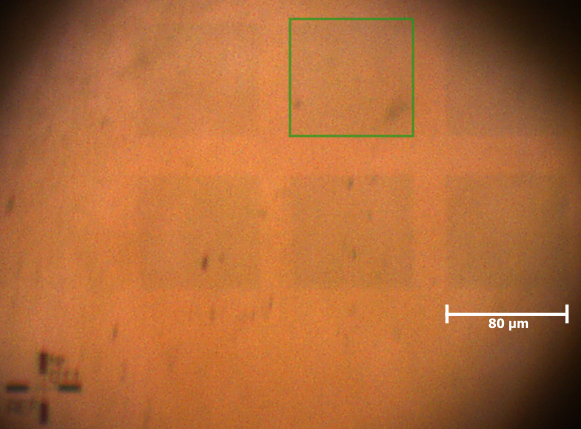
\includegraphics[width=0.43\textwidth]{Hell.png} }}
    \qquad
    \subfloat[\centering Dark-field image]{{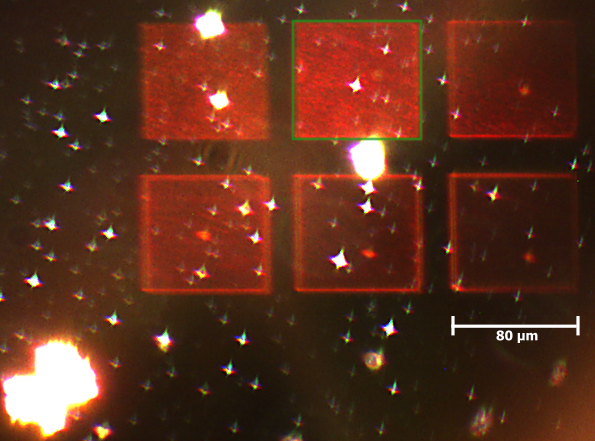
\includegraphics[width=0.43\textwidth]{DunkelBild.png} }}
    \caption{\label{fig:bilder}An image of the sample in bright-field mode, depicting light transmitted 
    through the sample (a), and in dark-field mode, illustrating light scattered by the sample (b). 
    The excitation light is non-polarized. A reference marker in the bottom left corner confirms 
    observation of the same areas of the sample.
    Additionally, a sample field has been marked in green, serving as a guide to the eye.}
\end{figure}\FloatBarrier 
Firstly, in both images, the sample fields are clearly visible, indicating that we have 
focused the sample well. 
Both pictures show the same sample section, making comparison easier. 
As mentioned, the bright-field microscopy image is mainly generated by the incident light. 
The darkened sample fields absorb or deflect the light, resulting in weaker transmission 
in those areas. 
Thus, a kind of shadow is obtained where interacting material is present. 
A significantly lower light intensity is required for capturing, 
but it is noticeable that the contrast to the background is lacking.
For thinner and smaller samples that interact weakly, no difference can be discerned 
in bright-field mode, and the signal is lost. \\ 
In dark-field mode, on the other hand, no direct incident light from the lamp reaches the camera. 
The signal is generated by scattered light from the samples or other particles. 
From the image, it can be observed that the contrast is significantly increased, 
and the sample fields are more clearly separated from the background. 
However, a stronger light intensity is required for measurement, allowing more light 
to be scattered and detected. 
Additionally, it is evident that impurities can lead to strong scattering. 
The bright points spread across the sample are particles on its surface that strongly scatter light, 
producing an additional unwanted signal. \\
In conclusion, it is evident for this type of sample that dark-field microscopy produces 
more beautiful images with better contrast, making it easier to associate the detected 
intensity with the actual sample. 
Nevertheless, the bright-field mode also works, and the choice of method depends 
on the sample under investigation. \newpage
Finally, let's consider the influence of light polarization. 
For this purpose, two images are captured in dark-field mode using linearly polarized light. 
The polarizer can be oriented parallel or perpendicular to the length of the nanorods. 
The comparison of the captured images is illustrated in Figure \ref{fig:polari}.
\begin{figure}[h!]
    \centering
    \subfloat[\centering Polarization angle $\alpha=0^{\circ}$]{{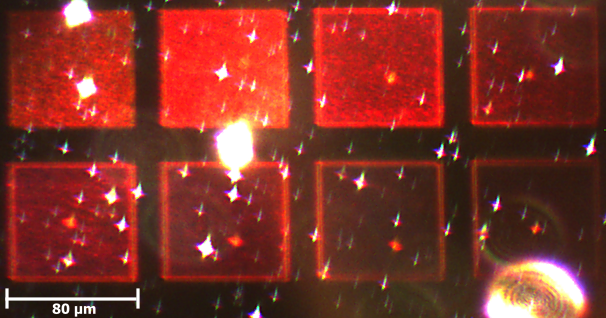
\includegraphics[width=0.47\textwidth]{Gruppe0.png}}}
    \qquad
    \subfloat[\centering Polarization angle $\alpha=90^{\circ}$]{{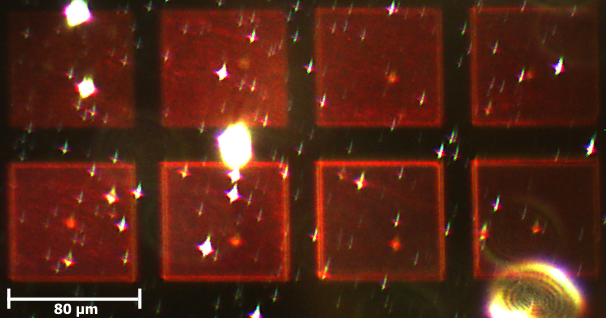
\includegraphics[width=0.47\textwidth]{Gruppe90.png} }}
    \caption{\label{fig:polari}A comparative image of a group of nanorod samples with constant width 
    and varying length. The groups were illuminated with differently linearly polarized incident 
    light, with the polarization angle $\alpha$ measured relative to the longitudinal orientation 
    of the nanorods.}
\end{figure}\FloatBarrier
For a polarization angle of $90^{\circ}$, no significant difference in color or intensity of the 
sample fields is apparent. 
In some cases, the field seems slightly darkened, but no systematic pattern is discernible. 
However, when the polarizer is set to $\alpha=0^{\circ}$, a systematic behavior of the sample 
fields becomes evident. 
It appears that the intensity seems to decrease or the color changes. 
This decrease starts in the upper left, moves to the upper right, 
and then continues from the lower left to the lower right. 
Referring to the sample layout in Fig.~\ref{fig:proben}, it is noticeable that in this sequence, 
the length of the nanorods increases. \\
This behavior can be explained through the excited plasmon modes. 
When the light is polarized perpendicular to the nanorod, the transverse mode is excited, 
utilizing the width $W$ of the nanorod as a resonator. 
In the considered group, this width remains constant, which is why the resonance 
wavelength does not change, and the scattered light looks comparable. 
When the light is polarized with $\alpha=0^{\circ}$ to the nanorods, 
the field excites electrons in the metallic silver nanoparticle to undergo 
a longitudinal oscillation. 
As the length of the rods, and thus the resonator length, changes per sample field, 
the resonance wavelength shifts, leading to an altered color perception in the image. 
This relationship is schematically depicted in Figure \ref{fig:long}.
\begin{figure}[h!]
    \centering
    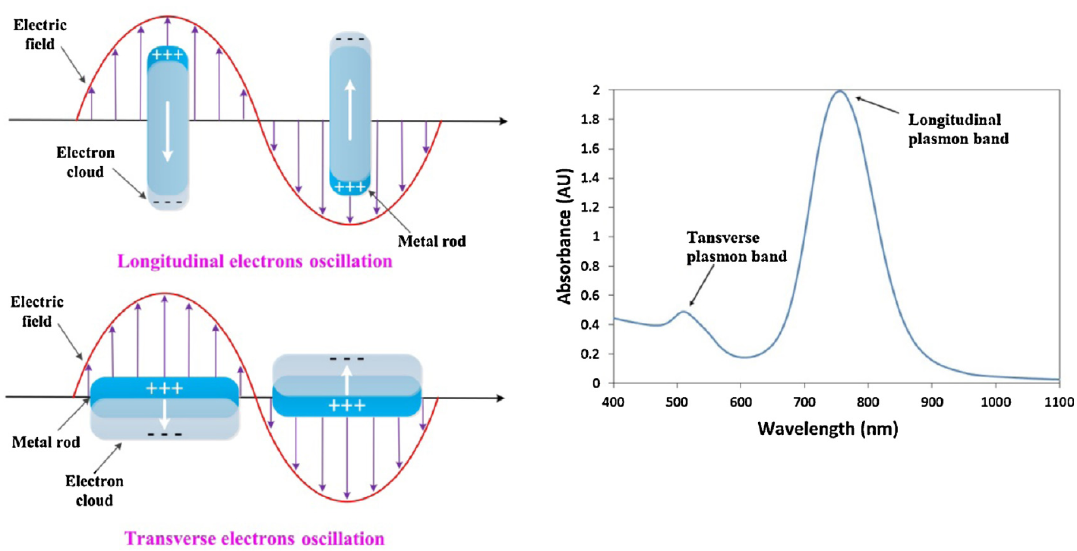
\includegraphics[width=0.6\textwidth]{long.png}
    \caption{\label{fig:long}A schematic representation of the different vibrational modes of the 
    plasmons on the nanorods. Illustrated are the transverse and longitudinal oscillations of 
    the electron clouds, excited depending on the polarization of the incident light. 
    The graphic is adapted from the experimental manual \cite{Anleitung}.}
\end{figure} \FloatBarrier
Overall, this qualitative observation confirms the assumption that the nanorods on the sample 
fields are not isotropically aligned but exhibit a preferred direction. In the following section, 
we will investigate this behavior using a spectrometer, allowing us to further determine the 
resonance wavelength and derive additional properties of the nanoparticles. \newpage



  